
%(BEGIN_QUESTION)
% Copyright 2006, Tony R. Kuphaldt, released under the Creative Commons Attribution License (v 1.0)
% This means you may do almost anything with this work of mine, so long as you give me proper credit

Shown here is a distillation tower, used to separate a liquid mixture of substances into its constituent components.  The process of {\it distillation}, or {\it fractionation} as it is sometimes called, is very common in heavy process industries, most notably petrochemical processing:
 
$$\includegraphics[width=15.5cm]{i01376x01.eps}$$

The light vapors extracted from the top of a distillation tower are recondensed into an ``accumulator'' vessel and re-introduced into the fractionation process as ``reflux.''  The heavy vapors condensing at the bottom of the tower are reboiled into vapor form again and re-introduced into the fractionation process as ``boil-up.''  It is necessary for reflux and boil-up to be re-introduced into the tower in order to purify the final products as much as possible.  The P\&ID shown here is devoid of any instrumentation for the sake of simplicity.

\filbreak

Here, a simple reflux control loop is shown, to control the amount of reflux introduced into the tower from the accumulator:

$$\includegraphics[width=15.5cm]{i01376x02.eps}$$

The tower operates at a controlled pressure of 75 PSI.  Reflux flows from the accumulator, through the valve, and into the tower by gravity alone.  The elevation difference between the accumulator's constant liquid level and the reflux control valve is 12 feet, and the reflux product is liquid pentane (specific gravity = 0.6262).  If a maximum reflux rate of 500 GPM is desired through this valve, what must its $C_v$ be?

\vskip 20pt \vbox{\hrule \hbox{\strut \vrule{} {\bf Suggestions for Socratic discussion} \vrule} \hrule}

\begin{itemize}
\item{} Identify some practical purposes for distillation towers in industry.
\item{} Which of the two heat exchangers {\it adds} heat to the tower?
\item{} Which of the two heat exchangers {\it removes} heat from the tower?
\item{} Suppose the liquid in the accumulator were something other than pentane (i.e. suppose the specific gravity was not equal to 0.6262).  How would this affect control valve sizing, assuming the same maximum flow rate of 500 GPM was desired?
\item{} Identify the effect(s) of the LT failing with a high signal (100\% liquid level) in this control system.
\item{} Identify the effect(s) of the LC being left unattended in manual mode in this control system.
\end{itemize}

\underbar{file i01376}
%(END_QUESTION)





%(BEGIN_ANSWER)

$C_v$ = 219.22
 
%(END_ANSWER)





%(BEGIN_NOTES)

$$\Delta P = \left(12 \hbox{ ft pentane} \over 1 \right)  \left(12 \hbox{ in} \over 1 \hbox{ ft}\right)  \left(1 \hbox{ PSI} \over 27.68 \hbox{ "WC}\right)  \left(0.6262 \hbox{ "WC} \over 1 \hbox{ "pentane}\right) = 3.258 \hbox{ PSID}$$

$$Q = C_v \sqrt{\Delta P \over G_f}$$

$$C_v = {Q \over \sqrt{\Delta P \over G_f}}$$

$$C_v = {500 \over \sqrt{3.258 \over 0.6262}} = 219.22$$

\vskip 10pt


Note that the valve's $\Delta$P is purely generated by the elevation head between the accumulator's level and the control valve.  The tower pressure of 75 PSI is of no concern to us in calculating this valve's capacity coefficient.

Interestingly, the liquid's density is of no concern to us either in this particular case, since gravity is the only force motivating its flow through the valve.  A simple thought experiment confirms this: try doubling the specific gravity and see what happens.  If $G_f$ doubles, the differential pressure drop across the valve resulting from 12 feet of elevation head doubles along with it.  However, so does the density term of the control valve $C_v$ formula, which means the value of the fraction inside the radicand ($\Delta P \over G_f$) remains constant regardless of the liquid's density.

%INDEX% Final Control Elements, valve: sizing
%INDEX% Process: distillation (pentane)

%(END_NOTES)


